% !TEX TS-program = pdflatexmk
% !TEX encoding = UTF-8 Unicode
% -------------------------- 
%  
%  SEM-ReadMe.tex : Alles, was man wissen sollte
%  Stand:	2023/01/27   
% 
% --------------------------
\documentclass[%
	,ngerman
%	,fontsize		= 12pt
	,DIV			= calc 
	,toc			= bib
	,abstract		= true
	,parskip		= half+
	,toc 		= numberline
%	,mydina4
		]{scrartcl}

%% -- Nutze die AGFA-Pakete
%% --
\usepackage[numeric,urldoi]{agfa-art}

%% -- Literatur
%% --
\addbibresource{CTAN.bib}
\addbibresource{TeX.bib}
\addbibresource{Artikel.bib}
\addbibresource{Buecher.bib}
%
\ExecuteBibliographyOptions{%
	,backref		= true		 	
	,url		= true	 	
	,doi		= false		
	,eprint		= false		
	}

%% -- Links farbig
%% --

\hypersetup{
	,colorlinks	= true    			%                                             
	,urlcolor	= blue       		%                                                              
	,citecolor	= blue      		    %                                                          
	,linkcolor	= blue			 	%  
%  	,hidelinks 						%  
	}
	
%% -- Titelseite
%% --
\title{Die Vorlage \texttt{SEM-Master.tex}}
\subtitle{-Erläuterungen-}
\date{\today}
\author{U. Groh}

%% -- Inhaltsverzeichnis kompremiert
%% --
%\RedeclareSectionCommands[tocraggedpagenumber,toclinefill={}]{section,subsection}
%\RedeclareSectionCommands[tocraggedpagenumber]{section,subsection}
\BeforeStartingTOC[toc]{\begin{multicols}{2}}
\AfterStartingTOC[toc]{\end{multicols}}

%% -- Für Listings etc.
%% --
\usepackage{ug-listings}

%\usepackage{2up}

%\targetlayout{booklet}

%% -- Start des Dokuments
%% --	
\begin{document}

%% -- Titel inkl. Abstract und Dictum

\maketitle
\tableofcontents
\thispagestyle{empty}

\dictum[\href{https://de.wikipedia.org/wiki/Friedrich_Dürrenmatt}{F. Dürrenmatt}]{Das Rationale am Menschen sind seine Einsichten, das Irrationale, dass er nicht danach handelt.}
%%
\begin{abstract}
Dies ist eine kleine Übersicht zu \TeX{}, der Nutzung von \LaTeX{} und Erläuterungen zu den Vorlagen.
Dies ist \enquote{keine} fehlerfreie Ausarbeitung und sie kann nur für einen ersten Einstieg sinnvoll sein.
Gern helfe ich aber, wenn es Probleme damit oder es Fragen zur Nutzung von \LaTeX{} gibt.
\end{abstract}

%% -- SEM-ReadMe-1.tex
%% --
% !TEX root = ../SEM-ReadMe.tex
%% -----------------------------
%% Stand: 2023/01/27
%% -----------------------------
\section{Etwas zu \LaTeX{}}
Um den Einstieg in \LaTeX{} etwas zu erleichtern, sind im Folgenden einige Punkte zusammengestellt, die für die ersten Schritte nützlich sind. 
Alles, was blau markiert ist, ist mit Links auf weiterführende Informationen hinterlegt.
Des Weiteren habe ich in einige \LaTeX{}-Tipps separat erstellt, die einiges vertiefen, was ich hier nur kurz anspreche -- diese finden sich auf ILIAS.

% 
\subsection{Was ist \LaTeX{}}
%\subsubsection{}
\LaTeX{} ist eine \href{https://de.wikipedia.org/wiki/Auszeichnungssprache}{Markup-Sprache}, die auf dem \href{https://de.wikipedia.org/wiki/Satz_(Druck)}{Textsatzsystem} \TeX{} basiert und ist, vor allem im naturwissenschaftlichen Bereich, zu einem \emph{de facto} Standard geworden.
Im Gegensatz zu den \href{https://de.wikipedia.org/wiki/WYSIWYG}{\emph{What You See is What You Get}} Systemen wie etwa Word, wird hier mittels Steuerelemente die Gestalt (Layout) des Dokuments festgelegt 
-- \href{https://de.wikipedia.org/wiki/WYSIWYM}{\emph{What You See is What You Mean}}.
Der Nutzer kann sich somit ganz auf den \emph{Inhalt} seiner Arbeit konzentrieren.
Dies ist zwar am Anfang etwas aufwendiger zu erlernen ist, aber es ist dadurch flexibler und besser auf die eigenen Bedürfnisse anpassbar.%
\footnote{Nebenbei: Word lernt man auch nicht über Nacht und für mathematischen Text ist dieses System weitestgehend unbrauchbar.}

Zur Geschichte von \TeX{} und die Gründe, warum es \href{https://de.wikipedia.org/wiki/Donald_E._Knuth}{Donald Knuth} vor über 50 Jahren geschaffen hat, findet man in seinem Buch \enquote{Digital Typography} \cite{knuth:digital} oder in \textcite{beeton:math}.
\href{https://de.wikipedia.org/wiki/LaTeX}{\LaTeX{}} selbst ist ein Makropaket, das auf \href{https://de.wikipedia.org/wiki/Leslie_Lamport}{L. Lamport} zurückgeht, der dieses um 1983 herum entwickelt hat -- siehe hierzu seine Erläuterungen in \cite{lamport:dmv}.

Eine gute Referenz für einen ersten Einstieg ist \textcite{lshort-german}, da sich hier alles Wesentliche zur Nutzung von \LaTeX{} findet.
Zu beachten ist aber, dass sich diese Einleitung auf \LaTeX{} des Jahres 2001 bezieht -- zwischenzeitlich ist einiges passiert, was die Eingabe erleichtert.
Dies betrifft vor allem die Eingabe eines Textes mit Zeichensätzen außerhalb des anglo-amerikanischen Sprachraums.
Trotzdem -- bitte unbedingt nutzen.

Als Literatur ist das RRZN-Handbuch \emph{ \LaTeX{}-—Einführung in das Textsatzsystem} zu empfehlen, das man leider über das hiesige Rechenzentrum der Universität Tübingen nicht beziehen kann.%
\footnote{Bei Interesse bin ich gern bereit eine Sammelbestellung zu initiieren.} 
Die Bücher von Herbert Voß -- siehe hierzu \url{https://www.dante.de/dante-e-v/literatur/} -- sind für alle empfohlen, die sich intensiver mit \LaTeX\ beschäftigen wollen.
Zu empfehlen ist \textcite{voss:2012a} \enquote{\citetitle{voss:2012a}} als Begleitlektüre.%
\footnote{Gut ist auch die Begleitdokumentation von Overleaf, das man sich via \texttt{Help} anzeigen lassen kann}

Für deutsche Texte sind die Dokumentenklassen, die auf KOMA-Script beruhen \textcite{kohm:2020}, da hier die Gegebenheiten bei uns berücksichtigt sind -- die Klassen von KOMA-Script werden in den Musterdateien genutzt.

\subsection{Wie startet man}
Zum Start bieten sich zwei Alternativen an:
%
\begin{myitemize}[nosep]
	\item 
	Eine lokale Installation auf seinen eigenen Laptop oder PC -- dies ist meine Empfehlung, wenn dies möglich ist.
	
	\item
	Die Nutzung des Onlineangebots Overleaf \url{https://de.overleaf.com} -- dazu das zip-File in Overleaf installieren
	(siehe hierzu die Anleitung zu der Vorlage).
	
\end{myitemize}
%
Zur lokalen Installation nutzt man die über die \TeX-Users Group (TUG) via \href{https://tug.org/texlive/}{TeX Live} zur Verfügung gestellt wird. 
Dies betrifft Systeme mit Windows oder Ubuntu und dieses wird gepflegt, \dh es gibt jährlich ein Update.

Wer zu den Glücklichen gehört, die einen Mac nutzen (mit OS X), für die steht eine auf TeX Live basierendes System zur Verfügung (\url{https://tug.org/mactex/}).
Dieses System beinhaltet auch einen sehr guten Editor, \href{https://pages.uoregon.edu/koch/texshop/}{TeXshop}, ein Verwaltungsprogramm für die Literatur, \href{https://bibdesk.sourceforge.io}{BibDesk} und eine Reihe von Tools, die einem das Erstellen von \TeX{}-Dokumenten erleichtert..
Einführung zu diesen Programmen findet man auch auf YouTube.

Wie erwähnt, arbeitet \TeX{} mit Steuerzeichen die \enquote{sagen}, was gemacht werden soll.
Man kann daher dieses System mit einer Programmiersprache vergleichen und es ist somit anfällig gegen Fehler bei der Eingabe dieser Steuerzeichen. 
Eine einfache Regel für den Anfang: Sparsam sein bei der Verwendung von Steuerzeichen und nicht verzweifeln im Fehlerfall.
Meistens stimmen die Klammern, speziell im Mathematikmodus, paarweise nicht!

\subsection{Bitte beachten}
%\subsubsection{}
%
Ein \enquote{\LaTeX{}-Sourcefile} besteht immer aus drei Teilen:

\begin{myenumerate} 
	\item 
	\emph{Aus der Präambel:} Dies ist alles zwischen \verb|\documentclass[..| und \par
	\verb|\begin{document}|.
	Hier finden sich (in der Regel) eigene Definitionen, der Aufruf von speziellen Paketen, die man als Ergänzung nutzt etc.
	Dazu einfach die Musterdatei und die Referenzen ansehen.
	
	\item
	\emph{Aus dem Hauptteil: } Nach dem \verb!\begin{document}! startet der Teil, der den Inhalt darstellt.
	Dieser wird entsprechend untergliedert und die einzelne Abschnitte mit Überschriften versehen.
	Wie man dieses machen kann -- siehe das Muster.
		
	\item
	\emph{Aus dem Schluss: } Dieser startet mit der Ausgabe der Literatur mittels der Umgebung für das Literaturverzeichnis -- \verb!\printbibiography! -- beinhaltet eventuell den Index \etc und endet mit \verb!\end{document}!.
	
	\item
	Nach der Umwandlung und wenn alles richtig ist, hat man ein PDF-Dokument mit einem optisch ansprechenden \href{https://de.wikipedia.org/wiki/Layout}{Layout}.
\end{myenumerate}
%
Ich habe ein kleines \LaTeX{}-File vorbereitet, das man für die ersten Gehversuche und die Erstellung der Ausarbeitung für die Hausarbeit nutzen kann.
Diese Vorlage ist aber für eine Bachelor- oder Masterarbeit nicht ausreichend, aber man kann diese als Basis nehmen und entsprechend \enquote{ausbauen}.%
\footnote{Ein Template für Bachelor- oder Masterarbeiten für AGFA findet sich auf GitHub unter \url{https://github.com/ugroh/AGFA-Master}}


\subsection{Einige Tipps }
Noch einige Tipps: 

\begin{myenumerate}
	\item
	Starte jeden neuen Satz auf einer neuen Zeile.
	Dies macht alles übersichtlicher und hilft, wenn man Fehler im Code sucht.
	Es ist \TeX{} kein System, mit dem man \href{https://de.wikipedia.org/wiki/Fließtext}{Fließtext} schreiben sollte.
	
	\item
	Bitte nicht \verb!\\! oder \verb!\newline! zu verwenden, um einen neuen Absatz zu erhalten.
	Will man einen neunen Absatz haben, so macht man dies mittels einer Leerzeile im laufenden Text.
	Den Rest -- Trennung nach den deutschen Regeln \ua -- macht dann das Programm.
	
	\item
	Wer sich unsicher ist, ob die Rechtschreibung oder die Zeichensetzung stimmt, der findet unter 
	\href{https://grammis.ids-mannheim.de}{https://grammis.ids-mannheim.de} Hilfe.
	Und es gibt sogar Programme, die einem bei der Erstellung von Texten helfen, etwa \href{https://languagetool.org/de}{LanguageTool}.
	Ganz zu schweigen von den KI-Tools wie \href{https://openai.com/blog/chatgpt/}{chatGTP }
	
	\item
	Nutze \textcite{lshort-german} für die ersten \enquote{Gehversuche} in \LaTeX\@.
	Aber bitte beachten: Es verwendet die Dokumentenklassen von \LaTeX{} als Beispiele, die aber nicht für die Eigenheiten der deutschen Sprache geeignet sind.
	Besser ist es mit KOMA-Script zu arbeiten, wie es in den Vorlagen gemacht wurde (\textcite{kohm:2020}).
	
	\item
	Es ist nicht mehr erforderlich, etwa Umlaute, durch spezielle Befehle einzugeben, wie es früher notwendig war.
	Wer seinen Editor korrekt auf UTF-8 eingestellt hat, kann einfach schreiben.
	
	\item
	Es gibt einige typographische Regeln, sowohl für die Eingabe eines Textes als auch für die Mathematik.
	Mehr dazu findet man unter \href{http://menetekel.e-technik.fh-muenchen.de/skripten/LaTeX/typokurz.pdf}{typokurz}, auf \href{https://www.typolexikon.de}{dem TypoLexikon Online} und unter \textcite{nadler:formelsatz} nützliche Tipps.
	
	\item
	Für den Einstieg in die Mathematik mit \LaTeX{} empfehle ich den AMS-Guide \cite{short-math-guide}.
	Weiteres findet man dann etwa in \textcite{graetzer:2007} oder in \textcite{voss:2012b}.	
	
	\item
	Zu empfehlen ist auch das Interview mit Leslie Lamport und seine drei Empfehlungen zu verinnerlichen (\cite{lamport:dmv})
	
	\item
	Alle diejenigen, die schon \LaTeX{} nutzen: Mal in \textcite{l2tabu} reinschauen.
	Dort finden sich alle Sünden, die man bei der Nutzung des Systems nicht machen soll.
	
		
\end{myenumerate}


%% -- SEM-ReadMe-2.tex
%% --
% !TEX root = ../SEM-ReadMe.tex
%% -----------------------------
%% Stand: 2022/10/10
%% -----------------------------
\section{Einige Empfehlungen}
\subsection{Eingabe des Textes}
%
Da in der Regel ein deutscher Text eingegeben wird, müssen auch die Regeln der deutschen Rechtschreibung und Zeichensetzung beachtet werden.
Dies wir mit dem Paket \texttt{babel} \cite{babel} erreicht:

\begin{enumerate}
\item
Richtige \enquote{Gänsefüßchen} mittels \verb|\enquote{...}|.

\item
Richtige Trennung, auch für das Wort \emph{Urinstinkt}.

\item
Richtige Eingabe von: siehe etwa \og oder \dh oder \etc \ldots
\end{enumerate}
%
Dies erreicht man mittels 
%\usepackage[babel,german=guillemets]{csquotes}
%\babelprovide[hyphenrules=ngerman-x-latest]{ngerman}
%
%\begin{tcolorbox}%lstlisting}{listing only}
%\cs{usepackage[ngerman]\brackets{babel}}
%\end{tcolorbox}
%
\begin{tcblisting}{listing only}
\documentclass[ngerman]{scrartcl}
\usepackage[ngerman]{babel}
\usepackage[austostyle,german=guillemets]{csquotes}
\babelprovide[hyphenrules=ngerman-x-latest]{ngerman}
...
\begin{document}
...
\end{document}
\end{tcblisting}
%%
Also etwa
%
\begin{tcblisting}{title= \enquote{Anführungszeichen Deutsch}}
Richtig: \enquote{Gänsefüßchen}
Und noch richtiger: \enquote{Gänsefüßchen und nochmals \enquote{Gänsefüßchen} im Text}
\end{tcblisting}
%
%In beiden Fällen kann man in eine andere Sprache umschalten, etwa von deutsch auf englisch:
%%
%\begin{tcblisting}{title= \enquote{Anführungszeichen Englisch}}
%\begin{otherlanguage}{english}
%Now we get \enquote{the right one.}
%Additionally: \enquote{Gänsefüßchen and once more \enquote{Gänsefüßchen} in the text.}
%\end{otherlanguage}
%\end{tcblisting}
%
Wer aber weitere Sprachen nutzen will, muss dieses entsprechend ergänzen.
Details hierzu und wie man umschaltet findet man im Manual zum Paket \lpkg{babel} unter 
\href{https://ctan.ebinger.cc/tex-archive/macros/latex/required/babel/base/babel.pdf}{babel.pdf} oder man schaut mal in \textcite[3.7.2]{voss:2012a} rein.
%
\subsection{Eingabe von Mathematik}\label{subsec:eingabe-mathe}
Einer der Stärken von \TeX{} ist die Eingabe mathematischer Ausdrücke, wie etwa
%
\[
	\frac{ a+b }{ c+ \frac{ 1 }{ d+e } }
\]
%
oder von mathematischen Umgebungen, wie etwa so:
%
\begin{theorem}\label{thm:hauptsatz}
%	
Ist $ f $ eine stetige reellwertige Funktion auf dem Intervall\/ $ \interval{0,1} $, so ist
%
\[
  	F( t ) = \int_{ 0 }^{ t } f(s) \ds
\]
%
differenzierbar auf diesem Intervall und $ F'(t) = f(t) $ für alle $ t \in \interval{0,1} $ .
\end{theorem}
%
Vor allem kann man später immer auf dieses Theorem über Querverweise einfach zurückgreifen, also \enquote{siehe \cref{thm:hauptsatz}} funktioniert (wenn man alles richtig gemacht hat).
Basis dazu ist das Paket \texttt{amsmath}, eine Entwicklung der American Mathematical Society \href{https://de.wikipedia.org/wiki/American_Mathematical_Society}{AMS}.

Auch hier, mehr noch als bei der Eingabe von reinem Text, gilt es sorgfältig zu arbeiten. 
Mein Tipp: \enquote{Platz lassen}, wie etwa bei der Eingabe des obigen Bruchs
%
	\begin{tcblisting}{title=Eingabe einer Formel, listing only}
		%
		\[
			\frac{a+b}{c + \frac{1}{d+e}}
		\]
		%
	\end{tcblisting}
%
Dies ist einfacher zu \enquote{lesen}, speziell, wenn es komplexer wird.
So sollte es jedenfalls nicht aussehen:
%
\begin{center}
	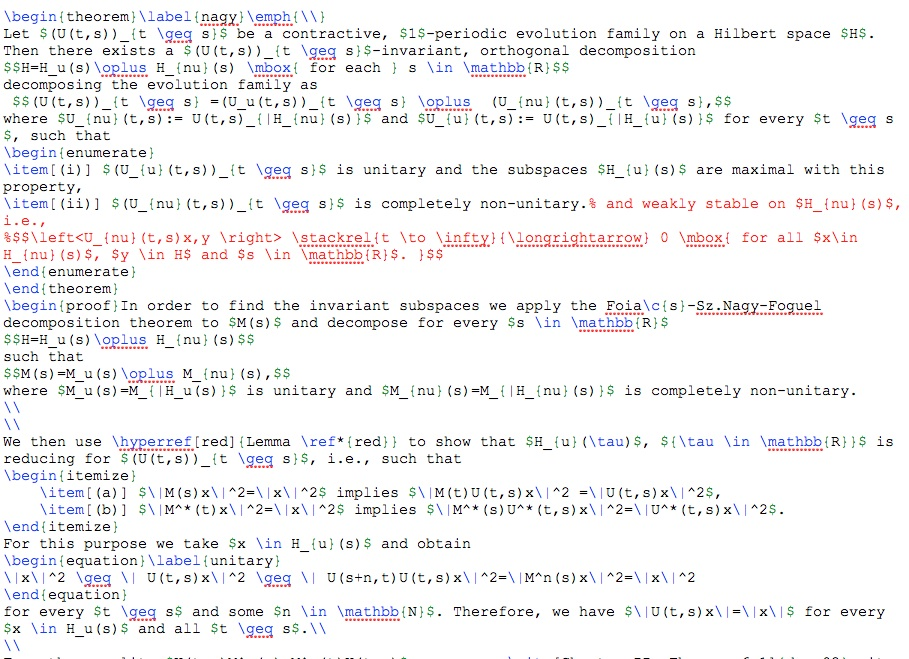
\includegraphics[scale=0.4]{./content/example2}
\end{center}
%
Am Anfang (und auch später) wird man öfters ein Buch zu Rate ziehen, wenn es um die Eingabe von speziellen Zeichen wie Integral $ \int $ oder Summen $ \sum_{ n = 1 }^{ \infty } r_{ n } $ geht.
Die Literatur und \href{http://tug.ctan.org/info/symbols/comprehensive/symbols-a4.pdf}{\LaTeX{}-Symbole} \cite{comprehensive} helfen dabei.
%Als Begleitliteratur für den mathematischen Teil empfehle ich das Buch \textcite{voss:2012b} oder \textcite{graetzer:2007}.
Ein nettes Hilfsmittel zum Üben und zum Erstellen mathematischer Formeln ist \href{https://www.chachatelier.fr/latexit/}{LaTeXit} -- leider nur für die Nutzer eines Apple Mac-Systems.

Noch ein Hinweis: Der Mathematikmodus hat zwei Varianten:
%
\begin{myitemize}
	
	\item
	Der \emph{Inline}-Modus via \verb!$ \alpha $! oder \verb|\( \alpha \)|: Beides ergibt \( \alpha \) in der Zeile (oder die Summe weiter oben).
	Ich denke, dass die Eingabe  mittels \verb|$ ... $| besser ist, da diese sich von den Klammern abhebt, die man in der Regel noch zusätzlich hat.
	
	\item
	Der \emph{abgesetzte Modus}: Siehe hierzu das Beispiel zu den Brüchen.
	Für diesen ist es \emph{verboten}, die Variante \verb!$$ ... $$! zu nutzen.
	Diese ist eine \sog Primitive aus dem Fundus von \TeX{} und schon seit den Zeiten der ersten Version von \LaTeX{} nicht mehr sinnvoll.
		
	\begin{tcblisting}{title=Abgesetzte Formel ohne Nummer}
		%
		\[
			\frac{a+b}{c + \frac{1}{d+e}}
		\]
		%
	\end{tcblisting}
	%%
		\begin{tcblisting}{title=Abgesetzte Formel mit Nummer}
		%
		\begin{equation}\label{eq:gleichung}
			\frac{a+b}{c + \frac{1}{d+e}}
		\end{equation}
		%
	\end{tcblisting}
\end{myitemize}
%%
Noch ein Hinweis, da ich dieses mehrfach gesehen habe: Die \texttt{align*}-Umgebung ist kein Ersatz für die beiden \og abgesetzten Umgebungen sondern -- wie der Name sagt.
Beispiele dazu findet man in dem bereits erwähnten AMS-Guide \cite{short-math-guide}.

%% --
Zu beachten ist auch, dass für die Eingabe eines mathematischen Textes typographische Regeln gelten.
Die wesentlichen:

\begin{myenumerate}
	\item
	Grundsätzlich kursiv werden einfache Variable $ x $, $ y $, mathematische Funktionen $ z = f(x) $ oder Indizes $ x_{ j } $ gesetzt.
	
	\item
	Aufrecht gesetzt werden alle Ziffern $ 1 23 $, mathematische Funktionen mit bestimmten Eigenschaften, etwa $  \sin(x) $, Maßeinheiten wie $ 12 \, \mathrm{kg} $ \etc

\end{myenumerate}
%
Weiteres findet sich im Detail in \textcite{voss:2012b} oder \textcite{nadler:formelsatz}.

Ein Beispiel:
%% --
\begin{tcblisting}{title = Nicht korrekt, lower separated=false}
$ ds^2=dx^2+dy^2+dz^2-c^2dt^2 $
\end{tcblisting}
%%
\vs 
%%
\begin{tcblisting}{title = Richtig, lower separated=false}
\renewcommand*{\d}[1]{\mathop{}\!\mathrm{d}{#1}}
%
$ \d{s}^{2} = \d{x}^{2} + \d{y}^{2} + \d{z}^{2} - c\d{t}^{2} $
\end{tcblisting}

%%
\subsection{Mathematische Umgebungen}
Für die Theoreme etc.\@ wird das Paket \texttt{amsthm} \cite{amsthm} verwendet.
Das Prinzip ist immer das gleiche: Man verwendet die Konstruktion der Umgebungen von \LaTeX{}{} und benennt diese.
Die Grundkonstruktion ist 
%
\begin{tcblisting}{title = Mathematische Umgebungen, listing only}
\begin{name}\label{key:kuerzel}
 ....
\end{name}
\end{tcblisting}
%
wobei mit \verb!\label{..}! ein Querverweis mit Hilfe von \verb|\ref{...}| ermöglicht wird (siehe hierzu den entsprechenden \LaTeX{}-Tipp).
%
\begin{tcblisting}{title = Ein Theorem}
\begin{theorem}
\[
 \int \ldots
\]
\end{theorem}
\end{tcblisting}
%
\begin{tcblisting}{title = Ein Korollar}
Text
%
\begin{corollary}
  Also ist \ldots
\end{corollary}
%
oder
%
\begin{cor}
  Also ist \ldots
\end{cor}
%
wer es kürzer will.
\end{tcblisting}
%
Diese Definitionen erfolgen normalerweise in der Präambel.
Da diese aber unübersichtlich wird, sind alle Definitionen in die Datei
%%
\begin{tcolorbox}
SEM-art.tex
\end{tcolorbox}
%
ausgelagert und dort -- neben anderen -- vordefiniert und können so gleich genutzt werden.
%
\begin{tcblisting}{listing only}
		\newtheorem{theorem}{Theorem}
		\newtheorem{thm}{Theorem}
		\newtheorem{corollary}[theorem]{Korollar}
		\newtheorem{cor}[theorem]{Korollar}
\end{tcblisting}
%
%und ist in unserem Fall bereits vordefiniert, siehe \vref{tab:ma-umgebungen} für die Möglichkeiten.
%In allen Editoren zur Eingabe der \TeX{}-Syntax gibt es die Möglichkeit, die Eingabeformate als Tasttaturkürzel abzulegen.
%Bitte hierzu die Dokumentation des verwendeten Editors nachlesen.
Wichtig ist es, die Umgebungen mit einem korrekten Label zu versehen, da man dann die Möglichkeit hat, einfach darauf zu verweisen.
Es sieht dann etwa so aus: \ldots der Hauptsatz (siehe \vref{thm:hauptsatz}) gibt \ldots .

Die Details hierzu sind in einigen Tipps beschrieben, den sich auf ILIAS befinden.

\subsection{Aufzählungen}
Für Aufzählungen in Theorem, Sätzen \etc -- aber nicht nur hier --  gelten grundsätzlich die folgende Regeln:
%
\begin{enumerate}[(1)]
	\item 
	Aufzählungen, die keine Äquivalenzen sind, werden grundsätzlich mit kleinen \emph{römischen} Ziffern gekennzeichnet (also (i), (ii), \dots).
Die Eingabe erfolgt mittels
%
	\begin{center}
		\begin{lstlisting}
 			\begin{enumerate}[(i)]
				\item ..
			\end{enumerate}
		\end{lstlisting}
 	\end{center}
	
	\item
	Äquivalenzen  werden grundsätzlich mit den kleinen Buchstaben gekennzeichnet, also (a), (b), \dots .
	Die Eingabe erfolgt mittels	
	%
	\begin{center}
		\begin{lstlisting}{listing only}
			\begin{enumerate}[(a)]
				\item ..
			\end{enumerate}
		\end{lstlisting}
	\end{center}
	%
	
%	\item
%	Nummerierungen (also (1), (2), \dots oder ähnliches) erfolgen mittels
%	
%	\begin{center}
%		\begin{lstlisting}
% 			\begin{enumerate}[(1)]
% 			
%				\item ..
%			\end{enumerate}
%		\end{lstlisting}
%	\end{center}
%	%
			
\end{enumerate}
%
Notwendig, damit dieses funktioniert, ist das Paket \texttt{enumitem} \cite{enumitem}, was aber geladen wird.
Wer mehr dazu wissen will, kann es sich mittels \verb!texdoc enumitem! anzeigen lassen -- oder auf \href{https://ctan.org/pkg/enumitem}{diesen Link} klicken -- in dem Musterfile ist es bereits integriert.
Ansonsten kann man dieses auch für Aufzählungen in einer normalen Textumgebung nutzen und entsprechend anpassen.
%% --
\subsection{Literaturverzeichnis}
Hier gibt es zwei Möglichkeiten: 

\begin{myitemize}

\item 
Die \enquote{normale} Variante über die in \LaTeX{} enthaltene Umgebung 
%
\begin{tcblisting}{ title=Literaturverzeichnis, listing only}
\begin{thebibliography}{99}
%
\bibitem{graetzer:2007} George Grätzer,  
\emph{More Math into \LaTeX{}}, Springer (2007)
\ldots
\end{thebibliography}
\end{tcblisting}
%
Dies findet sich in der Musterdatei als Beispiel und ist völlig ausreichend für die Arbeit im Rahmen der Hausarbeit (oder für Arbeiten mit wenig Literatur).
Bitte die Art und Weise der Eingabe von Referenzen in der Literatur, etwa in \textcite{voss:2012a} nachlesen.
	
	\item
	Für größere Literaturzitate und -Sammlungen nutzt man das Paket \texttt{biblatex}  \textcite{voss:2011}. 
	Wer wissen will, wie dies geht: Bitte in \textcite{latextipps6} reinsehen.	
\end{myitemize}
%
Nebenbei: Die Pflege einer Literaturdatenbank erfolgt entweder über \href{https://de.wikipedia.org/wiki/BibDesk}{BibDesk} für Mac-Nutzer oder sonst mit \href{https://de.wikipedia.org/wiki/JabRef}{Jabref} sonst.
Wichtig sind auch die richtigen Abkürzungen der mathematischen Reihen, bei denen ein Artikel erschienen ist.
Dabei hilft \href{https://images.webofknowledge.com/images/help/WOS/A_abrvjt.html}{diese Unterlage}.
%

\subsection{Beamer}
%\subsubsection{}
Zum Schluss noch ein Hinweis auf \href{https://de.wikipedia.org/wiki/Beamer_(LaTeX)}{Beamer}: Dies ist ein System, das auf \TeX{} und \LaTeX{} aufbaut und die Erstellung von Präsentationen ermöglicht.
Ich denke, alle kennen \emph{Powerpoint}, das aber nur bedingt im naturwissenschaftlichen Umfeld sinnvoll eigesetzt werden kann (wegen der mathematischen Ausdrücken).
Vielleicht eine Gelegenheit, im Rahmen von Vorträgen \emph{Beamer} zu probieren.

Eine kleine Vorlage ist beigefügt -- \texttt{SEM-Baemer.tex} -- und unter 
 \url{https://bit.ly/3XeXp6R} findet man eine (kleine große) Übersicht.
Darüberhinaus gibt es auch auf YouTube Einführungen dazu, übrigens auch zu \LaTeX{}.
Die Definitionen für die Vorlage finden sich unter \texttt{./preamble/Beamer-defn.tex} und können natürlich angepasst werden.
%%


%% -- SEM-ReadMe-3.tex
%% --
% !TEX root = ../SEM-ReadMe.tex
%% -----------------------------
%% Stand: 2023/01/27
%% -----------------------------
\section{Die Muster \TeX{}-Datei}
\subsection{Die Vorlagen}
Ich habe vier Dateien erstellt:

\begin{myitemize}
	
	\item
	\texttt{SEM-Muster.tex}: Diese dient als Vorlage für kleinere Ausarbeitungen, etwa für eine Hausarbeit oder für den Vortrag eines Proseminars oder eines Seminars. 
		Man darf nur diese Datei mit dem \LaTeX{}-Compiler bearbeiten. 
		Die anderen sind sog.\@ \texttt{include}-Dateien, die Makros enthalten.
		
	\item
	\texttt{SEM-Beamer.tex}: Eine Datei, mit der Sie sicherlich Ihren Vortrag mal konzipieren können.
	Einfach mal reinschauen.
	
	\item
	Im Unterverzeichnis \texttt{preamble} befinden sich:
	
	\begin{myenumerate}

	\item
	\texttt{SEM-art.tex}: Beinhaltet das Layout, einige Definitionen für mathematische Umgebungen etc.\@ 
	Details werden in \vref{tab:mathematisches} besprochen.. 
	
	\item
	\texttt{SEM-defn.tex}: Beinhaltet einige Definitionen für Abkürzungen \etc, siehe \vref{tab:generelles}.
	
	\item
	Für eigene Definitionen bitte die Datei \texttt{My-defn.tex} nutzen aber vorher in die beiden \og reinschauen, was wie definiert ist \bzw wird. 
	
	\end{myenumerate}
	
	diese werden via \cs{input}\brackets{name-der-datei} eingebunden.
	
	\item
	Im Unterverzeichnis \texttt{content} befinden sich die Dateien mit dem fachlichen Inhalt, die ebenso über \cs{input}\brackets{name-der-datei} eingebunden werden.
	In unserem Fall \texttt{./ug-Master.tex} unsere Ausführungen und ale weiteres Beispiel \texttt{./MeinText.tex}, in dem man seine eigenen Ausführungen eintragen kann (oder jeder andere Namen für die vorhandene Datei).
		
\end{myitemize}

Man kann den Inhalt von \texttt{./preamble} auch in das  \texttt{texmf}-Verzeichnis unter \texttt{latex} kopieren; dann hat man alles stets zur Verfügung.
Falls der Sinn des \texttt{texmf}-Verzeichnises nicht bekannt ist: Einfach \href{https://www.overleaf.com/learn/latex/Articles/An_introduction_to_Kpathsea_and_how_TeX_engines_search_for_files
\%23Table_listing_Kpathsea_.E2.80.9Cconfig_variables.E2.80.9D}{mal diese Übersicht dazu lesen}.
\begin{remark}
Ein Hinweis für Mac-User: Nach der Installation von \TeX{} gibt es unter \texttt{$\tilde{}$/Library} ein Unterverzeichnis \texttt{texmf/tex/latex}.
Dort gehören die beiden letzten Dateien hin und werden von \LaTeX{} gefunden.

Für Windows-Nutzer: Bitte unbedingt \href{http://texlive.tug.org/texlive/}{texlive} nutzen und \href{http://texlive.tug.org/texlive/windows.html}{die Anleitung lesen}.
\end{remark}
%
\begin{remark}
Für die Nutzer von Overleaf: Bitte über \texttt{Code} rechts oben die zip-File herunterladen und als neues Projekt nach Overleaf kopieren. 
Es wird dann ein Verzeichnis mit dem gleichen Namen angelegt und man kann die Dateien ohne weiteren Installationsaufwand nutzen.
\end{remark}
% ------------------
\subsection{Die Definitionen}\label{subsec:definitionen}
Folgendes ist vordefiniert und findet sich in der \texttt{SEM-defn.tex} Datei.%
\footnote{Die folgenden Tabellen sind mit dem Paket \texttt{longtable} \cite{longtable} gesetzt worden. 
Details hierzu findet man in dem \og Manual oder in \textcite{voss:2012a}.}
% ------------------------------------------------------------------------------
\begin{center}
  \begin{longtable}{@{} lcl @{}}
  \caption{Generelles}\label{tab:generelles} \\
%-
  \toprule
  Die Eingabe & ergibt die  & folgende Ausgabe \\ 
  \toprule
  \endfirsthead  
%-
  \multicolumn{3}{@{}l}{\small\ldots\emph{Fortsetzung}} \\
  \toprule
  Die Eingabe & ergibt die  & folgende Ausgabe \\ 
  \toprule
  \endhead
%-
  \multicolumn{3}{@{}r}{\small{\emph{Fortsetzung nächste Seite}}\ldots} \\
  \endfoot
  \endlastfoot
% ------------------------------------------------------------------------------
    \emph{Anführungszeichen:} \\
    \verb|\enquote{Text}| & $ \to $ & \enquote{Text} \\ 
    \verb|\enquote{\ldots\enquote{Text}\ldots}| & $ \to $ & \enquote{\ldots\enquote{Text}\ldots} \\ 
    \midrule 
    \emph{Abkürzungen:} \\
    \verb|\zB| & $ \to $ & \zB \\ 
    \verb|\dh| & $ \to $ & \dh \\
     \verb|\og| & $ \to $ & \og \\
    \verb|\etc| & $ \to $ & \etc \\
    \verb|\bzw| & $ \to $ & \bzw \\
    \midrule
    \emph{Bindestriche:} \\
    \verb|-| & $ \to $ & Cauchy-Schwarz \\
    \verb|--| & $ \to $ & 1--10 \\
    \verb|$ - x $ | & $ \to $ & $ - x $ \\
%    \verb|$ - x $\) $| & $ \to $ & \( - x \) \\
% ------------------------------------------------------------------------------
    \bottomrule
  \end{longtable}
\end{center}
% 
\begin{remark}
Bei den Abkürzungen muss nach dem ersten Punkt einer kleiner Abstand eingehalten werden (laut Duden).
Dies ist hier eingehalten worden.
\end{remark}

%
\begin{center}
  \begin{longtable}{@{} lcl @{}}
  \caption{Mathematisches}\label{tab:mathematisches} \\
%-
  \toprule
  Die Eingabe & ergibt die  & folgende Ausgabe \\ 
  \toprule
  \endfirsthead  
%-
  \multicolumn{3}{@{}l}{\small\ldots\emph{Fortsetzung}} \\
  \toprule
  Die Eingabe & ergibt die  & folgende Ausgabe \\ 
  \toprule
  \endhead
%-
  \multicolumn{3}{@{}r}{\small{\emph{Fortsetzung nächste Seite}}\ldots} \\
  \endfoot
  \endlastfoot
%% -----------------------------------------------
    \emph{Zahlenmengen:} \\
    \verb| \N | & $ \to $ & $ \N $ \\ 
    \verb| \Z | & $ \to $ & $ \Z $ \\
    \verb| \Q | & $ \to $ & $ \Q $ \\
    \verb| \R | & $ \to $ & $ \R $ \\
    \verb| \C | & $ \to $ & $ \C $ \\
    \verb| \K | & $ \to $ & $ \K $ \\
	\midrule
	\emph{Integral:} \\
    \verb| \ds | & $ \to $ & $ \ds $ \\
    \verb| \dt | & $ \to $ & $ \dt $ \\
    \verb| \dx | & $ \to $ & $ \dx $ \\
    \verb| \diff{\mu} | & $ \to $ & $ \diff{\mu} $ \\
    \verb| \d{\mu} | & $ \to $ & $ \diff{\mu} $ \\
	\midrule
	\emph{Variable:} \\
    \verb| \phi | & $ \to $ & $ \phi $ \\
    \verb| \epsilon  | & $ \to $ & $ \epsilon $ \\
    \verb| \rho | & $ \to $ & $ \rho $ \\
	\verb| \theta | & $ \to $ & $ \theta $ \\
	\verb| \leq | & $ \to $ & $ \leq $ \\
	\verb| \geq | & $ \to $ & $ \geq $ \\
	\midrule
	\emph{Sonstiges: } \\
	\verb| \abs{x} | & $ \to $ & $ \abs{x} $ \\
	\verb| \abs{} | & $ \to $ & $ \abs{} $ \\
	\verb| \norm{x} | & $ \to $ & $ \norm{x} $ \\
	\verb| \norm{} | & $ \to $ & $ \norm{} $ \\
	\verb| \norm*{\sum} | & $ \to $ & $ \norm*{\sum} $ \\
	\midrule
	\verb| \interval{a,b}}| & $ \to $ & $ \interval{a,b}  $ \\
	\verb| \rointerval{a,b}}| & $ \to $ & $ \rointerval{a,b}  $ \\
	\verb| \lointerval{a,b}}| & $ \to $ & $ \lointerval{a,b}  $ \\
	\verb| \ointerval{a,b}}| & $ \to $ & $ \ointerval{a,b}  $ \\
% -----------------------------------------------
    \bottomrule
  \end{longtable}
\end{center}
%%
\begin{remark}
Kleine Anmerkung: Mittels der Eingabe der Sternvariante von \cs{abs} oder \cs{norm} sich die Größe der Begrenzungen an den folgenden Text an.
Etwa
%
\begin{tcblisting}{}
%
\[
	\abs*{ \frac{1}{\frac{a}{b+c}} }
\]
%
oder
%
\[
	\norm*{ \frac{1}{\frac{a}{b+c}} }
\]
%
\end{tcblisting}
\end{remark}
%%
Für die mathematischen Umgebungen stehen folgende Abkürzungen zur Verfügung:
\begin{center}
  \begin{longtable}{@{} lcl @{}}
  \caption{Mathematische Umgebungen}\label{tab:ma-umgebungen} \\
%-
  \toprule
  Die Eingabe & ergibt die  & folgende Umgebung \\ 
  \toprule
  \endfirsthead  
%-
  \multicolumn{3}{@{}l}{\small\ldots\emph{Fortsetzung}} \\
  \toprule
  Der Schlüssel \emph{key} & ergibt die  & folgende Umgebung \\ 
  \toprule
  \endhead
%-
  \multicolumn{3}{@{}r}{\small{\emph{Fortsetzung nächste Seite}}\ldots} \\
  \endfoot
  \endlastfoot
% ------------------------------------------------------------------------------
    \texttt{theorem} oder \texttt{thm} & $ \to $ & Theorem \\ 
    \texttt{prop}, \texttt{proposition} oder \texttt{satz} & $ \to $ & Satz \\
    \texttt{cor}, \texttt{corollary} oder \texttt{korollar} & $ \to $ & Korollar \\
    \texttt{lem} oder \texttt{lemma} & $ \to $ & Lemma \\
	\texttt{defn} oder \texttt{definition} & $ \to $ & Definition \\
	\texttt{examp}, \texttt{beispiel} oder \texttt{example} & $ \to $ & Beispiel \\
	\texttt{rem} oder \texttt{note} & $ \to $ & Anmerkung \\
% ------------------------------------------------------------------------------
    \bottomrule
  \end{longtable}
\end{center}
%
\begin{tcblisting}{title= Ein Beispiel}
\begin{theorem}
\ldots
\end{theorem}
\end{tcblisting}
%
\subsection{Wo bekommt man Hilfe?}
%
Bei der Nutzung des Systems wird man immer wieder auf Probleme stoßen.
Vieles wird man selbst lösen können, da es sich meistens um Eingabefehler handelt.
Kommt man aber nicht weiter, so gibt es verschiedene Webseiten, auf denen man Hilfe bekommt

\begin{itemize}
\item
Für alle möglichen Fragen, Installation \ua: \url{http://projekte.dante.de/DanteFAQ/WebHome}
\item
Für technische Probleme: \url{https://tex.stackexchange.com}

\end{itemize}

Und dann kann noch Google nutzen -- aber Achtung: Nicht alles, was man dann findet ist sinnvoll.
Hier sollte man auf das Datum der Frage achten. 



% --------------------------
% \setcounter{unbalance}{5}		
\nocite{voss:2012a,lamport:1986}
\printbibliography
%\end{multicols}
%
\end{document}

1.3 Was ist denn nun LaTeX (und muss ich das wissen)?

LaTeX ist ein System zur Erstellung von Texten, das von Leslie Lamport entworfen wurde.Die Information in diesem Abschnitt basiert auf den Angaben in dem Buch „A Guide to LaTeX2ε“ von Helmut Kopka und Patrick Daly. Die genaue Quellenangabe finden Sie im Literaturverzeichnis des Benutzerhandbuches. Es basiert auf der Textsatz-Sprache TeX, die bereits Mitte der 70er Jahre von Donald Knuth entwickelt wurde. „TeX“ spricht man aus wie „Blech“, und manche halten es auch für etwas blechern. Das liegt aber daran, dass die wenigsten verstehen, was TeX eigentlich ist. TeX liest aus einer ASCII-Datei eine Reihe von Textsatzbefehlen und führt sie aus. Das ist etwas komplizierter als eine Schreibmaschine, aber bei weitem nicht so schwierig wie eine echte Schriftsatz-Maschine in einer Druckerei. Aber viele der Tricks der Schriftsetzer wurden von Knuth als Computer-Algorithmen formuliert und in TeX integriert, daher sehen seine Druckergebnisse so hervorragend aus. TeX erzeugt als Ausgabe eine Datei, die man als geräteunabhängig („device independent“, DVI) bezeichnet. Eine solche DVI-Datei kann von vielen Programmen, die dieses Format verstehen, gelesen und in andere Formate wie zum Beispiel PostScript oder PDF umgewandelt werden.

Wäre das bereits alles, TeX wäre nichts anderes als ein primitiver Textsetzer. Aber in TeX ist es möglich, eigene Befehlssequenzen, so genannte Makros, zu definieren. Und dadurch sind die Möglichkeiten von TeX schier unbegrenzt.

Leslie Lamports Idee

Die meisten Leute, die TeX verwenden, benutzen tatsächlich ein Makropaket, das Knuth zusammengestellt hat, um den Großteil der Details beim Zeichensatz vor dem Anwender zu verstecken. Dieses Makropaket ist meist gemeint, wenn man von TeX spricht. Das eigentliche TeX mit seinen expliziten Satzbefehlen benutzt kaum ein normaler Anwender, das machen nur diejenigen Leute, die selber Makropakete entwickeln. Und hier kommt Leslie Lamport ins Spiel. Er wollte ein Makropaket, das sich näher am Benutzer orientiert, und nicht an den Feinheiten beim Textsatz. Ein Paket, mit dem sich einfach Dinge wie Abschnitte, Tabellen oder mathematische Formeln schreiben lassen, ohne zu verwirrend zu sein. So wurde LaTeX geboren. 

Parallel zur Weiterentwicklung von LaTeX entstanden andere, spezielle Pakete für TeX: Eines, um Folien zu schreiben oder eines, um Artikel für mathematische Zeitschriften zu erstellen, und so fort. Einige der Autoren verwendeten dazu TeX, andere begannen, LaTeX abzuändern. Um dieses Wirrwarr zu vereinfachen, begann eine Gruppe von LaTeX-Experten (zu denen natürlich auch Lamport selbst gehörte) in den späten 80er Jahren, LaTeX2ε zu entwickeln, die heutige Version von LaTeX. Diese neue Version stellt auch Befehle zur Verfügung, um neue Makros einfach zu erstellen, andere Zeichensätze zu definieren und so weiter. Alles in allem ist LaTeX dadurch selber eine ziemlich umfangreiche Sprache geworden. Überall auf der Welt haben Benutzer ihre eigenen Erweiterungen für LaTeX geschrieben.

Klassen und Stile

Es existieren zwei unterschiedliche Wege, wie man LaTeX erweitern kann: Klassen und Stile. Eine Klasse besteht aus einer Reihe von LaTeX- (und TeX-) Makros, die eine neue Art von Dokument beschreiben, wie etwa ein Buch oder einen Artikel. Es gibt zum Beispiel Klassen für Folien, für Artikel in mathematischen oder physikalischen Zeitschriften… Viele Universitäten haben sogar eigene Klassen für ihre Dissertationen zusammengestellt! Im Gegensatz dazu definiert ein Stil keine neue Art von Dokument, sondern eine anderes Verhalten, das ein Dokument nutzen kann.

So nutzt LyX zwei unterschiedliche Stil-Dateien, um die Ränder und Zeilenabstände in den Dokumenten festzulegen. Es existieren Stil-Dateien für fast jeden denkbaren Zweck: Um Etiketten und Umschläge zu beschriften, den Texteinzug zu verändern, um Grafikdateien handhaben zu können, spezielle Kopf- und Fußzeilen zu erstellen, Literaturlisten den eigenen Wünschen anzupassen, Erscheinungsbild und Position von Fußnoten, Tabellen und Abbildungen zu verändern und so weiter und so fort. Hier eine kurze Zusammenfassung:

00.00.0000 TeX: Makrofähige Programmiersprache für Schriftsatz.

00.00.0000 LaTeX: Makropaket auf der Basis von TeX.

00.00.0000 Klasse: Beschreibung eines Dokumententyps, verwendet LaTeX. 

00.00.0000 Stil: Verändert die Standardeinstellungen von LaTeX. 

00.00.0000 LyX: Visuelle WYSIWYM-Textverarbeitung, die LaTeX mit all seinen Fähigkeiten zum Ausdruck verwendet.

Der Zweck dieses Abschnittes war es, Ihnen zu zeigen, warum LyX etwas anders arbeitet als andere Textverarbeitungen. Der Grund ist einfach: LyX verwendet LaTeX als Formatierprogramm für den Ausdruck. Wie auch LaTeX konzentriert sich LyX auf den Inhalt Ihres Textes — also was Sie schreiben. Der Rechner kümmert sich dann darum, dass es gut aussieht.

Ach ja — eine letzte Bemerkung. LaTeX spricht man aus wie TeX, das sich auf das Wort Blech reimt. Laut Lamport kann man LaTeX auch „Läitech“ aussprechen. Wer es so ausspricht wie das Material, aus dem Kondome hergestellt werden, spricht es falsch. LyX dagegen spricht man „Lücks“. Oder „Licks“ — je nachdem, aus welchem Land man stammt.